\documentclass{article}
\usepackage[utf8]{inputenc}
\usepackage{graphicx}
\usepackage{cleveref}

\title{Big Programming Exercise \\ 
Implement the arctan function via ODE representation}
\author{Hasse Hansen}
\date{April 2019}

\begin{document}

\maketitle

\section{Introduction}
My exercise was to implement the arctagent function based on the derivative and a initial condition, which are as follows:
\begin{equation}
    \mathrm{arctan}'(x)= \frac{1}{x^2 + 1},
\end{equation}
\begin{equation} 
    \mathrm{arctan}(0)=0.
\end{equation}
To solve this I used the GSL function odeiv2, which solves the Ordinary Differential Equation (ODE), that is our derivate and initial condition. I placed the derivative equation in function of it self, such that another function, $myarctan$, could set that function as the ODE to solve. I used the Runga-Kutta-Fehlberg method since it was recommened on the GSL website, to be a good general solving method. The initial condition was then set and the ODE solver applied to the function. 

To make this function as general as possible, I call the myarctan function in a for loop, for different x values. In \cref{fig:arctan}, I have used x from 0 to 3, which is then plotted along side the arctan function from math.h. And it is quite clear, that my arctan function is sufficiently good to reproduce the arctan function from math.h. 



\begin{figure}
    \centering
    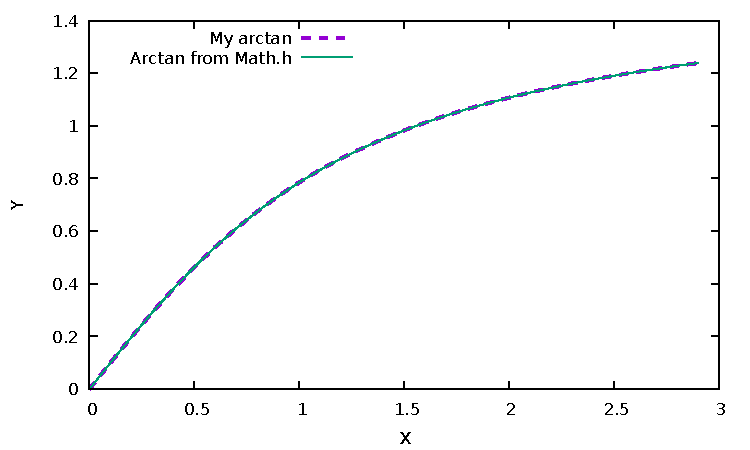
\includegraphics[width = \linewidth]{Atan.pdf}
    \caption{A plot of my arctan function and the arctan function from math.h}
    \label{fig:arctan}
\end{figure}

\end{document}
